\section{Simulation Results}

The proposed approach was validated in Gazebo under a ROS2 framework. A system of differential-drive robots was deployed in a planar workspace, with all agents initialized at random positions. The parameters used in each experiment are summarized in the corresponding tables.

\subsection{Average Consensus with Collision Avoidance}

\begin{figure*}[t]
    \centering
    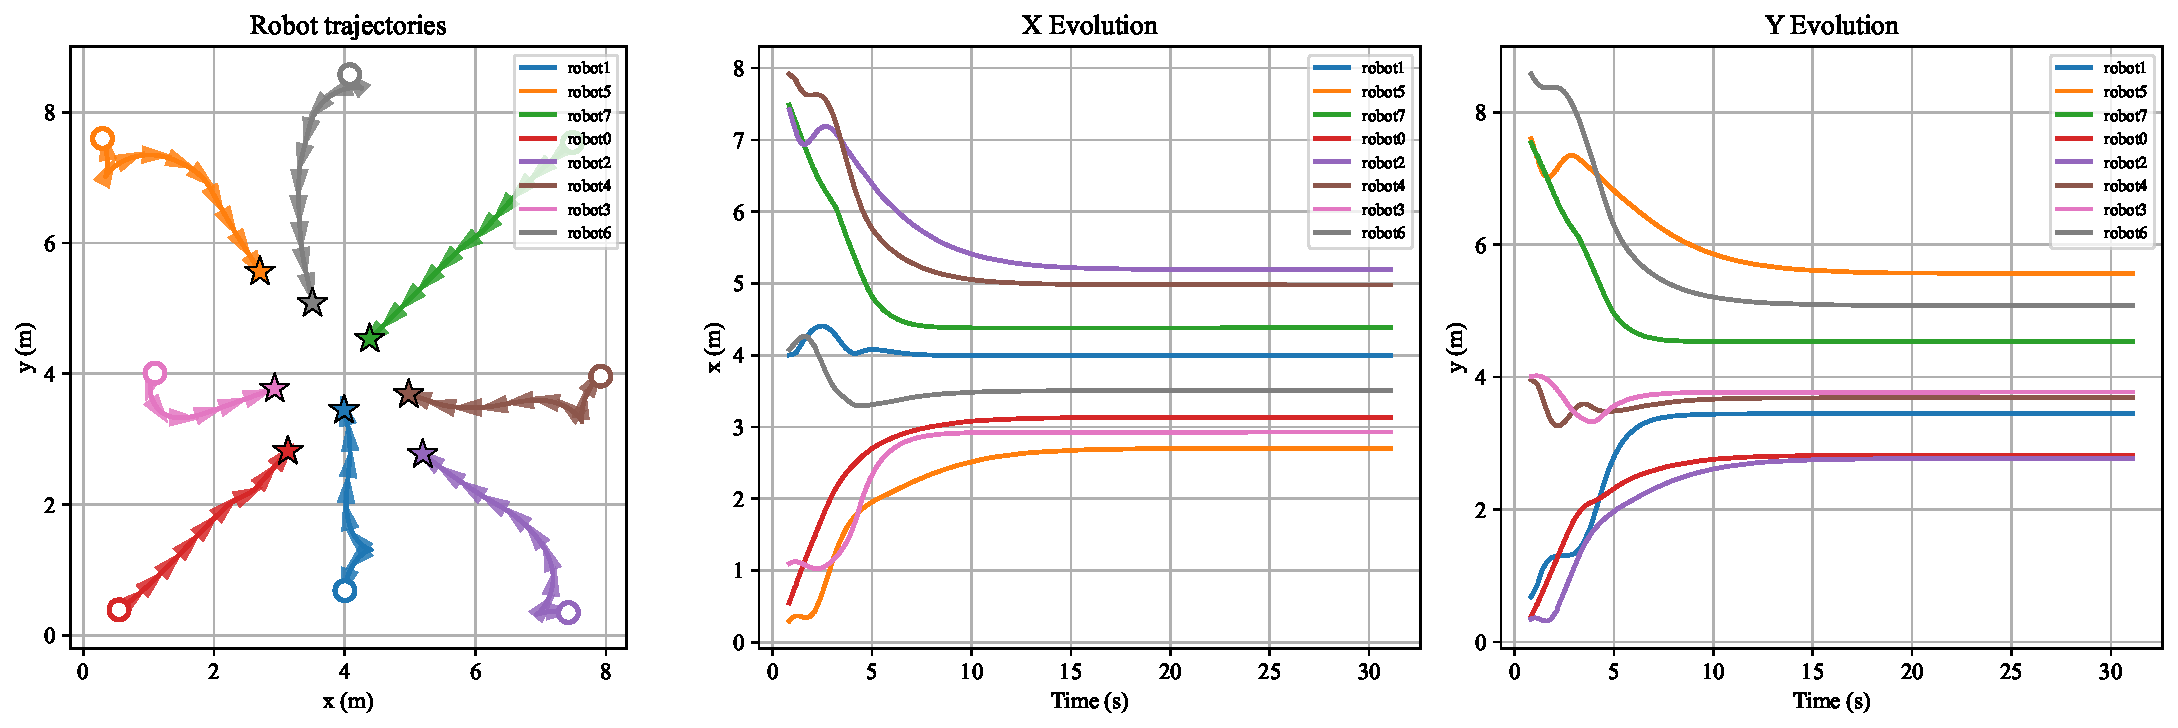
\includegraphics[width=\textwidth]{Pics/posiciones_finales.pdf}
    \caption{Simulation results for the average consensus experiment with $N = 8$ differential-drive robots. Robot trajectories (left) and time evolution of the $x$ and $y$ coordinates (center and right). All agents converge toward the average of their initial positions while the FVP module ensures collision-free trajectories throughout the motion.}
    \label{fig:consensus_results}
\end{figure*}

\begin{table}[h]
\centering
\caption{Parameters for the average consensus experiment}
\label{tab:params}
\begin{tabular}{lll}
\hline
\textbf{Parameter} & \textbf{Symbol} & \textbf{Value} \\
\hline
Linear gain & $k_1$ & $0.8$ \\
Angular gain & $k_2$ & $1.0$ \\
Maximum linear velocity & $v_{\max}$ & $1.0$ m/s \\
Maximum angular velocity & $\omega_{\max}$ & $1.0$ rad/s \\
Influence distance & $d_{\iota}$ & $3.0$ m \\
Safety distance & $d_s$ & $0.85$ m \\
Convergence coefficient & $\xi$ & $1.0$ \\
Sensor offset & $\|\mathbf{r}_p\|$ & $0.25$ m \\
\hline
\end{tabular}
\end{table}

The experiment considers $N = 8$ differential-drive robots randomly distributed in a workspace of approximately $8 \times 8$ m. Each robot updates its reference velocity from the consensus error defined in~\eqref{eq:consensus_error}, which quantifies the position disagreement with respect to its active neighbors. This reference is subsequently projected onto $\text{FVP}_i$, ensuring that the executed velocities are admissible with respect to the neighboring agents detected by the LiDAR sensor. As observed in Fig.~\ref{fig:consensus_results}, all robots converge toward the average of their initial positions in approximately 30 s, preserving collision-free trajectories throughout the process. The time evolution plots confirm the asymptotic convergence of both coordinates toward a common value, consistent with the diffusion dynamics induced by the proposed consensus protocol.

\subsection{Leader-Following with Collision Avoidance}

\begin{figure*}[t]
    \centering
    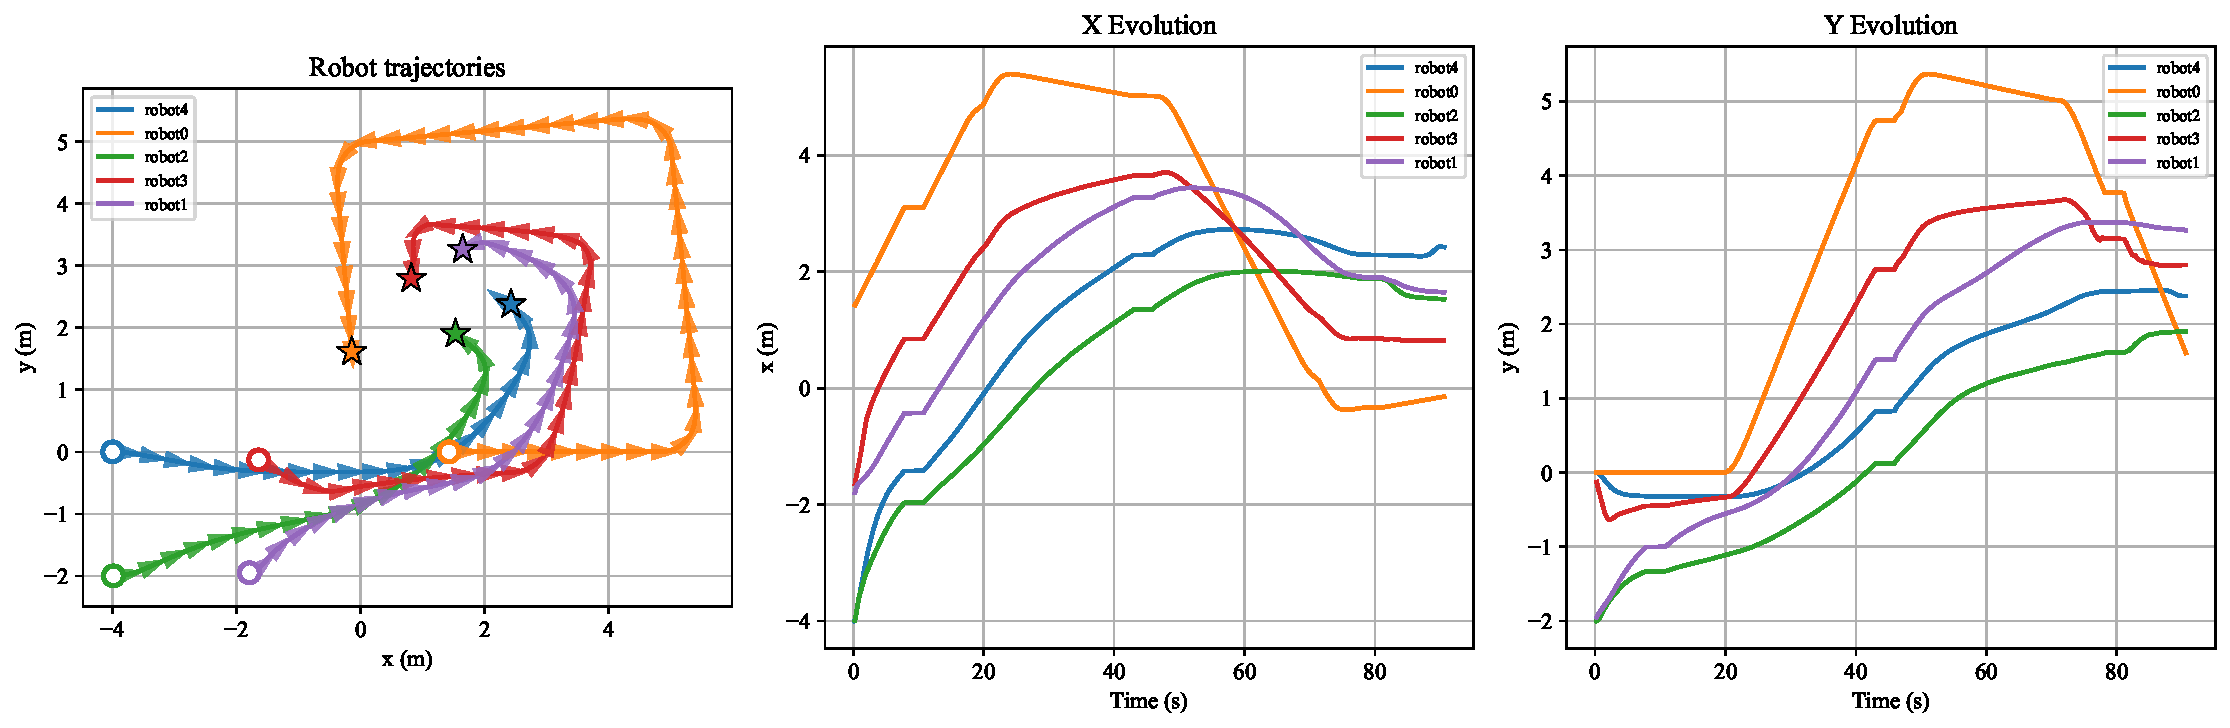
\includegraphics[width=\textwidth]{Pics/posiciones_finales_lider.pdf}
    \caption{Simulation results for the leader-following experiment with $N = 5$ differential-drive robots. The leader (robot0) traverses a $5 \times 5$ m square trajectory while the followers converge toward its position via the proposed consensus protocol. Stars indicate the final positions of each agent.}
    \label{fig:leader_results}
\end{figure*}

\begin{table}[h]
\centering
\caption{Parameters for the leader-following experiment}
\label{tab:params_leader}
\begin{tabular}{lll}
\hline
\textbf{Parameter} & \textbf{Symbol} & \textbf{Value} \\
\hline
Linear gain & $k_1$ & $1.5$ \\
Angular gain & $k_2$ & $1.5$ \\
Leader attraction gain & $k_L$ & $1.0$ \\
Maximum linear velocity (followers) & $v_{\max}$ & $0.8$ m/s \\
Maximum angular velocity (followers) & $\omega_{\max}$ & $0.8$ rad/s \\
Maximum linear velocity (leader) & $v_{\max}^{(0)}$ & $0.25$ m/s \\
Maximum angular velocity (leader) & $\omega_{\max}^{(0)}$ & $0.5$ rad/s \\
Waypoint tolerance & $\varepsilon$ & $0.15$ m \\
\hline
\end{tabular}
\end{table}

The experiment considers $N = 5$ differential-drive robots, where robot0 acts as the leader and the remaining four as followers. The leader sequentially traverses the vertices of a $5 \times 5$ m square defined by the waypoints $(5,0) \to (5,5) \to (0,5) \to (0,0)$, starting from the origin with orientation $\theta_0 = 0°$. The consensus error of each follower $i \in \mathcal{S}$ incorporates both the influence of its neighbors and the attraction toward the leader position:

\begin{equation}
    \mathbf{e}_i =
    \frac{1}{|\mathcal{N}_i|} \sum_{j \in \mathcal{N}_i}
    \begin{bmatrix} x_j - x_i \\ y_j - y_i \end{bmatrix}
    + k_L
    \begin{bmatrix} x_0 - x_i \\ y_0 - y_i \end{bmatrix}
    \label{eq:leader_error}
\end{equation}

\noindent where $k_L > 0$ is the attraction gain toward the leader and $(x_0, y_0)$ is its current position. As shown in Fig.~\ref{fig:leader_results}, the leader traverses the square trajectory while the followers are pulled toward its position, reactively adapting their trajectories to the leader's direction changes. The time evolution plots reflect the progressive convergence of the followers toward the leader state, with a transient of approximately 90 s associated with the length of the trajectory and the imposed velocity limits.

\subsection{Formation Maintenance with Leader Following}

\begin{figure*}[t]
    \centering
    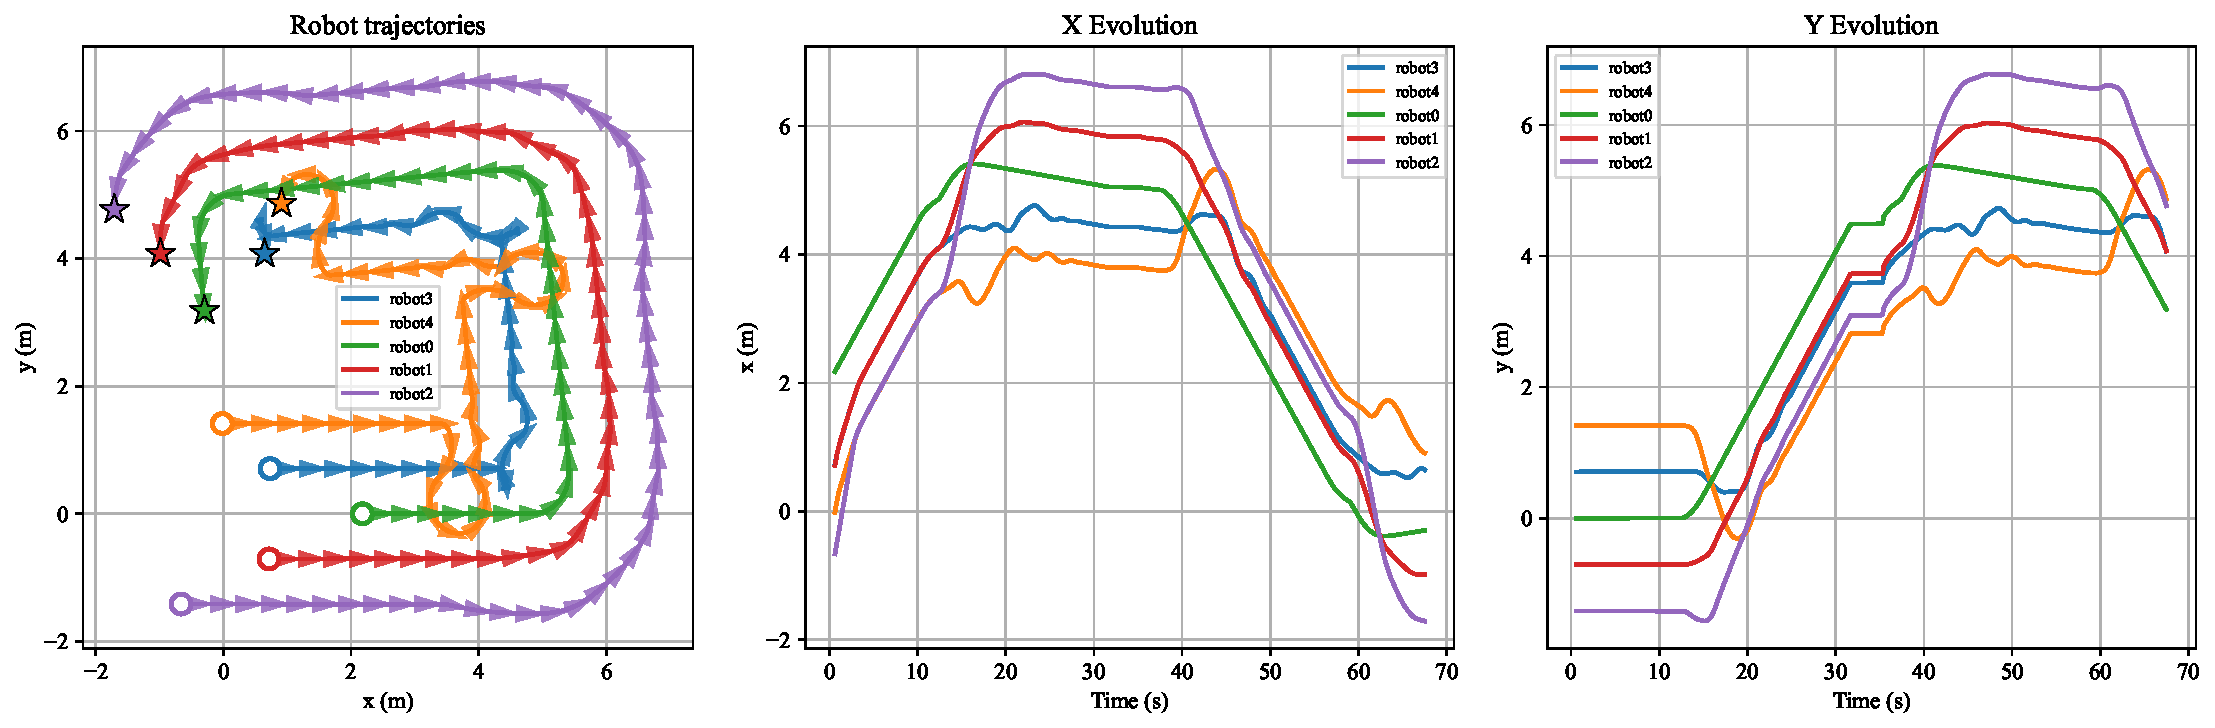
\includegraphics[width=\textwidth]{Pics/posiciones_finales_formación.pdf}
    \caption{Simulation results for the V-formation maintenance experiment with $N = 5$ differential-drive robots. The leader (robot0) traverses a $5 \times 5$ m square trajectory while the followers preserve the desired formation geometry via the protocol~\eqref{eq:formation_error}. Stars indicate the final positions of each agent.}
    \label{fig:formation_results}
\end{figure*}

\begin{table}[h]
\centering
\caption{Parameters for the formation maintenance experiment}
\label{tab:params_formation}
\begin{tabular}{lll}
\hline
\textbf{Parameter} & \textbf{Symbol} & \textbf{Value} \\
\hline
Linear gain & $k_1$ & $1.0$ \\
Angular gain & $k_2$ & $1.5$ \\
Anchor attraction gain & $\beta$ & $2.0$ \\
Leader orientation filter & $\gamma$ & $0.05$ \\
Maximum linear velocity (followers) & $v_{\max}$ & $0.8$ m/s \\
Maximum angular velocity (followers) & $\omega_{\max}$ & $0.8$ rad/s \\
Maximum linear velocity (leader) & $v_{\max}^{(0)}$ & $0.25$ m/s \\
Maximum angular velocity (leader) & $\omega_{\max}^{(0)}$ & $0.5$ rad/s \\
Waypoint tolerance & $\varepsilon$ & $0.15$ m \\
\hline
\end{tabular}
\end{table}

\begin{table}[h]
\centering
\caption{V-formation offsets at steady state ($\theta_L = 0$)}
\label{tab:offsets}
\begin{tabular}{llll}
\hline
\textbf{Robot} & \textbf{Arm} & \textbf{Level} & $\mathbf{r}_i$ (m) \\
\hline
robot1 & left  & 1 & $(-0.707,\ +0.707)$ \\
robot2 & left  & 2 & $(-1.414,\ +1.414)$ \\
robot3 & right & 1 & $(-0.707,\ -0.707)$ \\
robot4 & right & 2 & $(-1.414,\ -1.414)$ \\
\hline
\end{tabular}
\end{table}

The experiment considers $N = 5$ differential-drive robots under a leader-follower topology, where robot0 sequentially traverses the vertices of a $5 \times 5$ m square defined by the waypoints $(5,0) \to (5,5) \to (0,5) \to (0,0)$.

The formation offsets $\mathbf{r}_i$ are computed dynamically by rotating a fixed arm vector by the leader's filtered orientation $\theta_L$, with opening angle $\varphi_V = \pi/4$ and inter-robot spacing $d = 1.0$ m, as detailed in Table~\ref{tab:offsets}. 

A low-pass filter with coefficient $\gamma = 0.05$ is applied to $\theta_L$ to avoid abrupt offset updates at direction changes.

Each follower updates its state via the modified protocol~\eqref{eq:formation_error}, where the consensus term operates on offset-shifted positions $(\mathbf{x}_i - \mathbf{r}_i)$, guaranteeing that the desired formation is an exact equilibrium. As observed in Fig.~\ref{fig:formation_results}, the followers preserve the V-formation geometry throughout the leader's trajectory, reactively adapting to direction changes. The time evolution plots of both coordinates reflect the joint system dynamics, with a transient of approximately 70 s associated with the trajectory length and the imposed velocity limits.